\subsection{Global compositionality}
\label{subsec:global_compositionality}

In our final test, we focus on exceptions to compositional rules.
In natural language, typical exceptions that constitute a challenge for local compositionality are \emph{idioms}.
For instance, the idiom ``raining cats and dogs'' should be treated globally to arrive at its meaning of heavy rainfall.
A local approach would yield an overly literal, non-sensical translation (``het regent katten en honden'').
When a model's translation is too local, we follow \citet{hupkes2020compositionality} in saying that it \textbf{overgeneralises}, or, in other words, it applies a general rule to an expression that is an exception to this rule.
Overgeneralisation indicates that a language learner has internalised the general rule \citep[e.g.][]{penke2012dual}.

\subsubsection{Experiments}
We select 20 English idioms for which an accurate Dutch translation differs from the literal translation from the English MAGPIE corpus \citep{haagsma2020magpie}.
Because acquisition of idioms is dependent on their frequency in the corpus, we use idioms with at least 200 occurrences in OPUS based on exact matches, for which over 80\% of the target translations does not contain a literal translation.

\paragraph{Test design}
Per idiom, we extract \textit{natural} sentences containing the idiom from OPUS. 
For the synthetic and semi-natural data types, we insert the idiom in 500 samples per idiom per template, by attaching a subordinate clause to a noun -- e.g.\ ``the king \emph{that said `I knew the formula \textbf{by heart}'}''. 
The clauses used can be found in Appendix~\ref{ap:global_compositionality}, Table~\ref{tab:overgeneralisation_appendix}.

\paragraph{Evaluation}
Per idiom, we assess how often a model overgeneralises and how often it translates the idiom globally. 
To do so, we identify keywords that indicate that a translation is translated locally (literal) instead of globally (idiomatic).
If the keywords' literal translations are present, the translation is labelled as an overgeneralised translation. 
For instance, for ``by heart'', the presence of ``hart'' (``heart'') suggests a literal translation. An adequate paraphrase would say ``uit het hoofd'' (``from the head'').
See Appendix~\ref{ap:global_compositionality}, Table~\ref{tab:overgeneralisation_appendix}, for the full list of keywords.
We evaluate overgeneralisation for ten intermediate training checkpoints.

\begin{figure}
    \centering
    \begin{subfigure}[b]{\columnwidth}\centering
    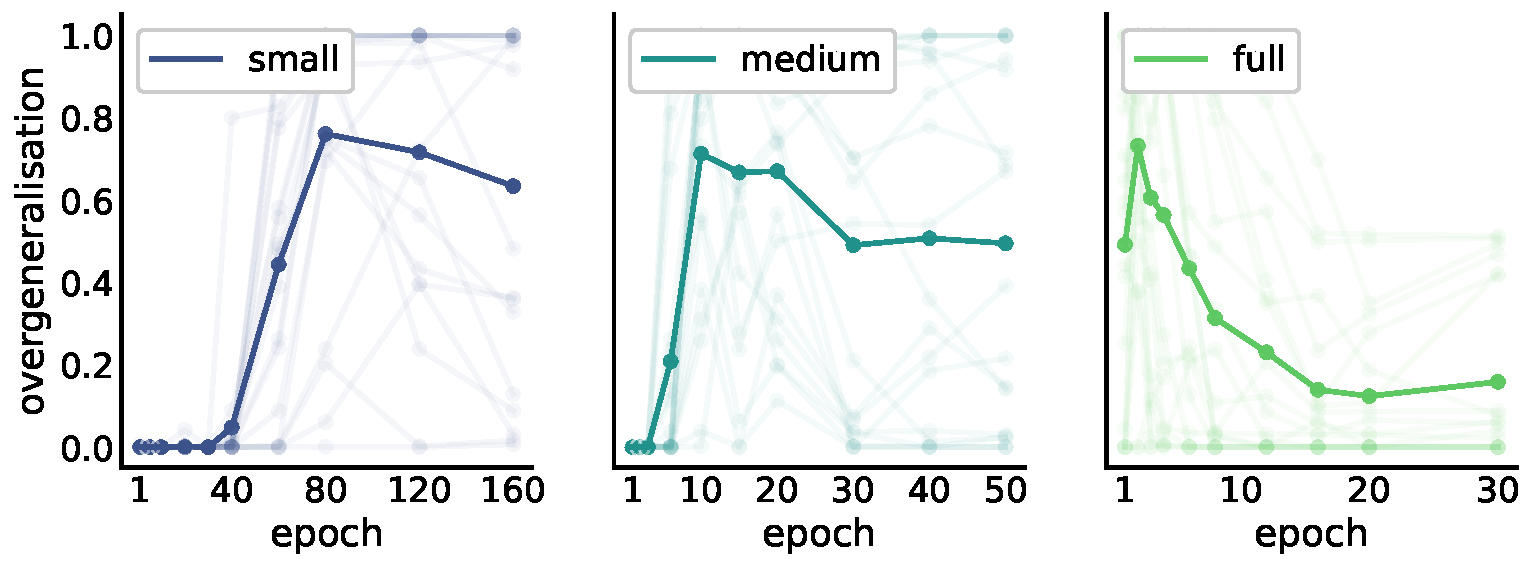
\includegraphics[width=\textwidth]{figures/global_compositionality/synthetic.pdf}
    \caption{Synthetic}
    \end{subfigure}
    \begin{subfigure}[b]{\columnwidth}\centering
    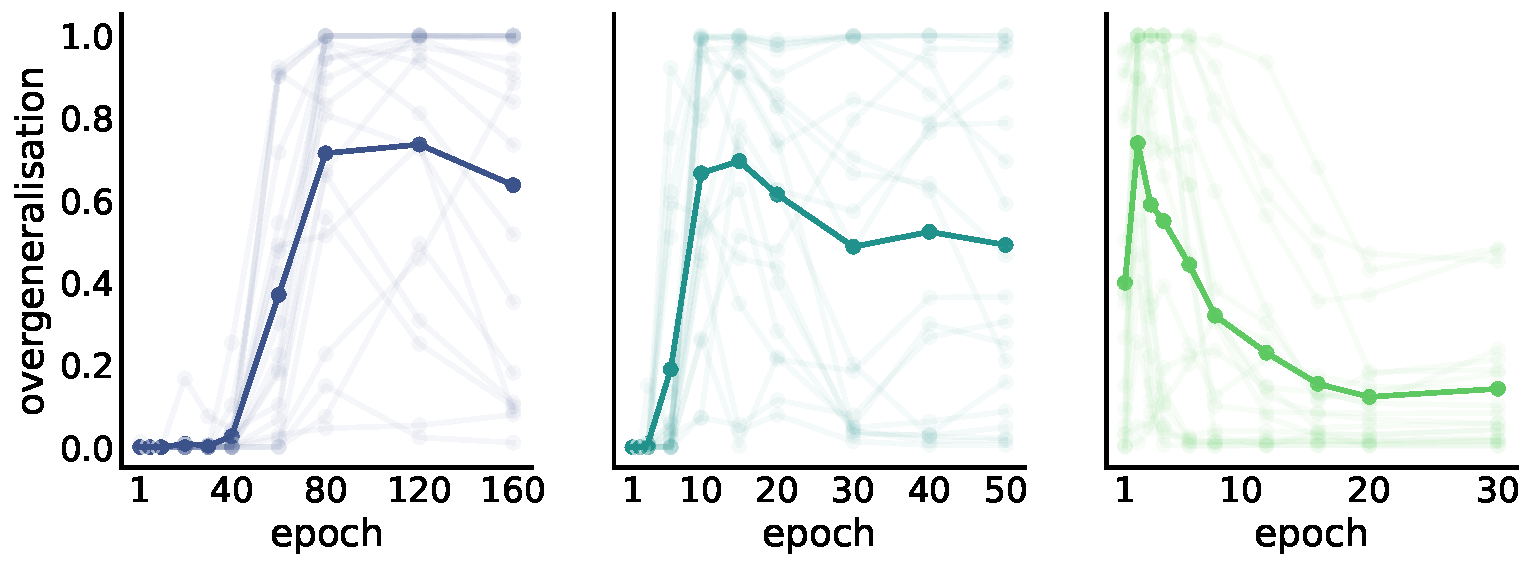
\includegraphics[width=\textwidth]{figures/global_compositionality/semi_natural.pdf}
    \caption{Semi-Natural}
    \end{subfigure}
    \begin{subfigure}[b]{\columnwidth}\centering
    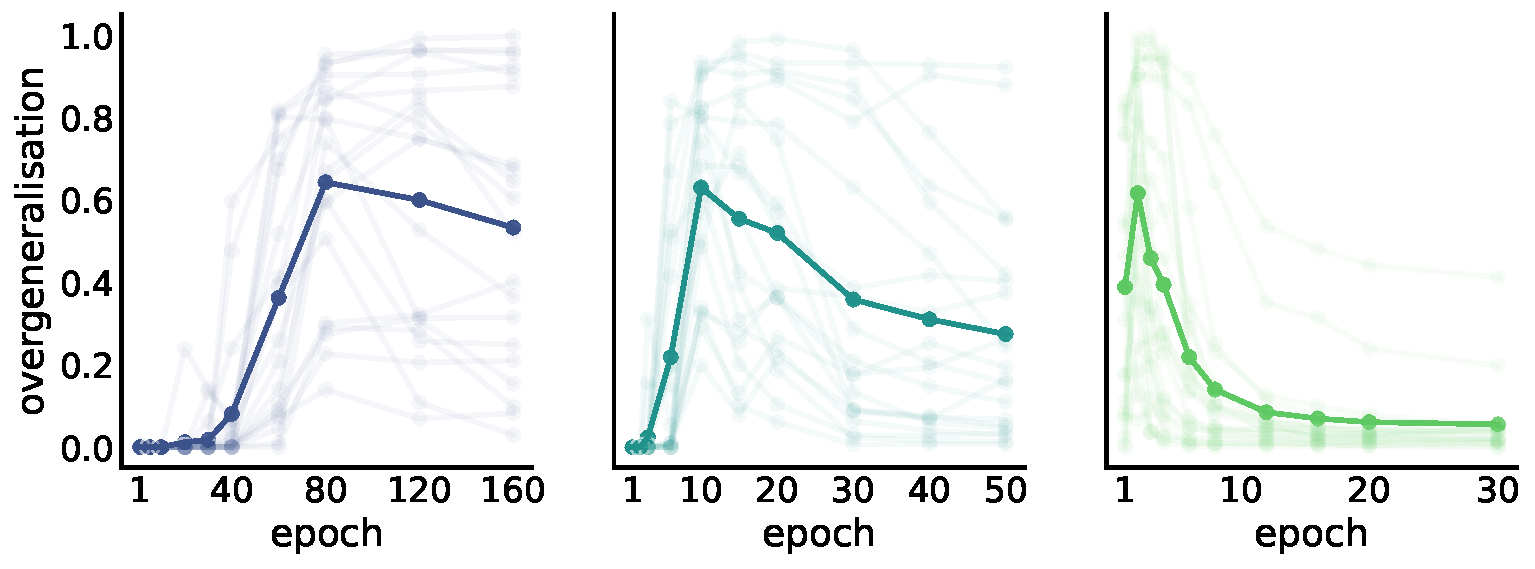
\includegraphics[width=\textwidth]{figures/global_compositionality/natural.pdf}
    \caption{Natural}
    \end{subfigure}
    \caption{Visualisation of overgeneralisation for idioms throughout training, with a line per idiom and the overall mean. Overgeneralisation occurs early on in training and precedes memorisation of idioms' translations.
    The colours indicate different training dataset sizes.}
    \label{fig:global_compositionality}
    \vspace{-0.3cm}
\end{figure}

\subsubsection{Results}
In Figure~\ref{fig:global_compositionality}, we report our results.\footnote{Note that epochs consist of different numbers of samples: 1M, 8.6M and 69M for small, medium and full. Appendix~\ref{ap:global_compositionality} further details numerical results per idiom.}
For all evaluation data types and all training set sizes, three phases can be identified.
Initially, the translations do not contain the idiom's keyword, not because the idiom's meaning is paraphrased in the translation, but because the translations consist of high-frequency words in the target language only. 
Afterwards, overgeneralisation peaks: the model emits a very literal translation of the idiom.
Finally, the model starts to memorise the idiom's translation.
This is in accordance with results from \citet{hupkes2020compositionality}, and earlier results presented in the past tense debate by -- among others -- \citet{rumelhart1986learning}.

Although the height of the overgeneralisation peak is similar across evaluation data types and training set sizes, overgeneralisation is more prominent in converged models trained on smaller datasets than it is in models trained on the full corpus.\footnote{Convergence is based on BLEU scores for validation data.}
In addition to training dataset size, the type of evaluation data used also matters: there is more overgeneralisation for synthetic and semi-natural data compared to natural data, stressing the impact of the context in which an idiom is embedded.
The extreme case of a context unsupportive of an idiomatic interpretation is a sequence of random words. To evaluate the hypothesis that this yields local translations, we surround the idioms with ten random words.
The results (Appendix~\ref{ap:global_compositionality}, Table~\ref{tab:overgeneralisation_appendix}) indicate that, indeed,  when the context provides no support at all for a global interpretation, the model provides a local translation for nearly all idioms.
Overall, the results of this test provide an interesting contrast with our substitutivity and systematicity results: where in those tests, we saw processing that was \emph{less local} than we expected, here, the behaviour shown by the models is instead \emph{not global enough}.